\chapter{Optimisation du choix de la matrice d'itération}
Nous avons vu dans la partie précédente qu'il existe différentes méthodes pour permettre de résoudre un système linéaire grâce à des méthodes itératives. Ainsi, toujours dans cette idée d'optimisation que nous avons exposé, nous nous sommes posé la question suivante : \og Quelle est la matrice d'itération la plus optimisé pour résoudre un problème \fg. Une méthode est ressortie dans plusieurs ouvrage : Successive Over Relaxation.
\section{Méthode SOR}
C'est dans cette optique que nous nous sommes penchés sur la méthode dite "SOR".
\subsection{Présentation de la méthode SOR}
La méthode SOR (Successive Over Relaxation) est une méthode itérative dérivée de Gauss-Siedel. En effet, le processus de décoposition de la matrice $A$ en deux matrices $M$ et $N$ telles que $A=M-N$ est similaire à l'algorithme de Gauss-Seidel dans la forme des matrices $M$ et $N$.\\

Si la méthode de Gauss-Seidel, vue précédemment, définie la matrice $M$ par $M=D-E$ avec $D$ une matrice diagonale et $E$ une matrice triangulaire inférieure à diagonale nulle et $N=F$, $F$ étant une matrice triangulaire supérieure à diagonale nulle, la méthode SOR définit ses matrices de la manière suivante, en introduisant un paramètre $\omega \in \mathbb{R}^*$ dit de relaxation.
\begin{eqnarray}
M &=& \frac{1}{\omega}D-E\\
N &=& \bigg(\frac{1}{\omega}-1\bigg)D+F
\end{eqnarray}
Par la suite, le procédé est le identique à celui de Gauss-Seidel ou Jacobi et on introduit donc sa matrice d'itération notée $B$.
\begin{equation}
B=M^{-1}N=\bigg[\frac{1}{\omega}D-E\bigg]^{-1}\bigg[\bigg(\frac{1}{\omega}-1\bigg)D+F\bigg]
\end{equation}
On remarquera que si $\omega=1$, on retrouve la méthode de Gauss-Seidel. De plus, si $\omega<1$, on parle de sous-relaxation et de sur-relaxation dans le cas où $\omega>1$.
\subsection{Intérêt de la méthode}
Cette méthode a été développée peu après la Seconde Guerre mondiale afin de proposer une manière de résoudre des systèmes d'équations linéaires, spécifique aux ordinateurs. Si à l'époque, d'autres méthodes avaient été proposées, elles étaient principalement destinées aux êtres humains qui, par des processus non applicables par des ordinateurs, pouvaient assurer la convergence des méthodes. La méthode SOR est donc une méthode qui a fait progresser ce problème en ayant une meilleure vitesse de convergence que les méthodes numériques itératives alors utilisées.\\

L'avantage de la méthode SOR au niveau de la convergence est mathématiquement facilitée par les deux théorèmes suivant:
\begin{enumerate}
	\item \textbf{\underline{Théorème de Kahan (1958)}} : Le rayon spectral de la matrice de relaxation, donnée par :
	$$
	T_\omega=T(\omega)=(I-\omega L)^{-1}{\omega U +(1-\omega)I}
	$$
	vérifie que $\forall \omega \neq 0$,
	$$
	\rho(T_\omega)\geq|\omega -1|
	$$
	\item \textbf{\underline{Théorème d'Ostrowski-Reich (1949-1954)}} : Si la matrice $A$ est définie positive et que $\omega \in ]0;2[$,la méthode SOR converge pour tout choix de vecteur $x^{(0)}$ initial.
\end{enumerate}
Afin qu'une méthode itérative converge, il est nécessaire que le rayon spectral de la matrice d'itération soit strictement inférieur à $1$. Donc, pour que la méthode ne converge pas, il faut que le rayon spectral soit supérieur ou égal à 1. Avec le théorème de Kahan, on a :
$$
|\omega -1|\geq 1 \Leftrightarrow \omega \geq 2 \text{ ou } \omega \leq 0 
$$
Ainsi, nous pouvons déduire du premier théorème, une condition nécessaire non suffisante de la convergence de la méthode SOR qui est :
\begin{equation}
0<\omega<2
\end{equation}
Le deuxième théorème (Ostrowski-Reich), permet quant à lui de conclure par rapport à la convergence de la méthode pour $\omega$ dans l'intervalle $]0;2[$. La combinaison de ces deux théorèmes nous montre que la condition donnée à l'équation $(3.4)$ est nécessaire et, est suffisante dans le cas où $A$ est définie positive.\\

De plus, dans le cas où la matrice $A$ est tridiagonale (les coefficients qui ne sont ni sur la diagonale principale, ni celle au dessus, ni celle au dessous, sont nuls), le théorème suivant nous donne la forme du coefficient de relaxation optimal :\\

Si $A$ est définie positive et est tridiagonale, alors $\rho(T_g)=[\rho(T_j)]^2<1$ et, le choix optimal pour le coefficient de relaxation $\omega$ est donné par : 
$$
\omega_{optimal}=\frac{2}{1+\sqrt{1-[\rho(T_j)]^2}}
$$
Avec ce choix de coefficient de relaxation, on a : $\rho(T_\omega)=\omega-1$\\
La preuve de ce théorème est dans : Ortega, J. M., Numerical
Analysis; A Second Course, Academic Press, New York, 1972, 201 pp.\\
\underline{\textbf{Preuve du théorème de Kahan}} : On a,
$$
\prod\limits_i \lambda_i(T(\omega))=\det(T(\omega))=\frac{\det(\omega U+(1-\omega)I)}{\det(I-\omega L)}=(1-\omega)^n 
$$
Or,
$$
|\prod\limits_i \lambda_i(T(\omega))|\leq\rho(T(\omega))^n \\
\rightarrow |\omega-1|^n\leq\rho(T(\omega))^n\\
$$
Ainsi,
$$
\rho(T(\omega))\geq|\omega-1|
$$
\underline{\textbf{Preuve du théorème d'Ostrowski-Reich}} : En utilisant le théorème de Kahan,on sait qu'il est nécessaire que  $0<\omega<2$ est un critère nécessaire et non suffisant de convergence. De plus, pour une méthode SOR, on a 
$$
M_{SOR}(\omega)+M_{SOR}^*(\omega)-A=\bigg(\frac{2}{\omega-1}\bigg)D \text{ puisque }L=U^*
$$
qui est symétrique définie positive si on est dans l'intervalle donné par le théorème de Kahan. Le théorème de Householder-John nous dit que pour une matrice $A$ hermitienne définie positive, avec $A=M-N$ avec $M$ inversible, la méthode itérative converge pour toute donnée initiale si $M+N^*$ est définie positive. ($N^*$ étant la matrice adjointe ou transconjugée à $N$ soit $N^*=^t\overline{N}=\overline{^tN}$).\\

Afin d'optimiser l'algorithme, on utilise souvent la méthode SSOR (Symetric Successive Over-Relaxation) afin de préconditionner la matrice avant de la traîter, cette méthode sera traîtée ultérieurement dans la partie optimisation.
\subsection{Implémentation numérique}
\section{Les espaces de Krylov}
\subsection{Présentation théorique}
\subsubsection{De Jacobi à Krylov}
On rappelle le résultat de la partie précédente sur la méthode de jacobi qui s'écrit : 
\begin{equation}
x^{k+1} = -D^{-1}(L+U)x^k + D^{-1}b = (I - D^{-1}A)x^{k} + D^{-1}b
\end{equation}
avec la matrice $A$ du système qui se décompose comme : $A = D + L + U$, $L$ une matrice triangulaire inférieur, $U$ un matrice triangulaire supérieur et $D$ diagonale. La matrice A est inversible car le système est supposé avoir une unique solution. On définit ensuite le résidu du système qui est par définition : 
\begin{equation}
r^k \triangleq b - Ax^k = -A ( - A^{-1}b + x^k) = -A (- x^* + x^k)
\end{equation}
Où $x^*$ est la solution réel du système. En normalisant le système ci-dessus de tel sorte que $D = I$. Alors, nous pouvons écrire la solution au rang k+1, comme celle au rang k plus le résidu : 
\begin{eqnarray}
x^{k+1} &=& x^k + r^k\\
\Leftrightarrow x^{k+1} - x^* &=& x^k - x^* + r^k\\
\Leftrightarrow -A( x^{k+1} - x^*) &=& -A(x^k - x^*) - Ar^k\\
\Leftrightarrow r^{k+1} &=& r^k - Ar^k
\end{eqnarray}
Dans cette dernière équation récursive, nous pouvons voir que $r^{k+1}$ est une combinaison linéaire des vecteurs $r^k$ précédents. Ainsi :
\begin{equation}
r^k \in Vect\{r^0, Ar^0, ..., A^kr^0\}
\end{equation}
Cela implique directement : 
\begin{equation}
x^k - x^0 = \sum_{i = 0}^{k-1}r^i
\end{equation}
Donc il vient que : 
\begin{equation}
x^k \in x^0 + Vect\{r^0, Ar^0, ..., A^kr^0\}
\end{equation}
Où $Vect\{r^0, Ar^0, ..., A^kr^0\}$ est le k-ème espace de Krylov généré par A à partir de $r^0$ noté $\mathcal{K}_k(A, r^0)$
\subsubsection{De nouvelles propriétés}
Maintenant que nous avons une définition de ces espaces, nous allons montrer plusieurs propriétés pour ensuite construire l'algorithme afin de l'implémenter. Le premier fait remarquable des espaces de krylov est que par construction, nous avons :  
\begin{equation}
\mathcal{K}_{k - 1}(A, r^0) \in \mathcal{K}_k(A, r^0)
\end{equation}
Ensuite, il est important de montrer que la solution que l'on cherche appartient à cet espace. Nous reprenons donc notre système linéaire possédant une unique solution : 
\begin{equation}
Ax = b \label{pb}
\end{equation}
D'après la définition du problème, la matrice A est inversible. Nous supposons que l'on a le polynôme caractéristique de A :
\begin{equation}
P(\lambda) = \sum_{j = 0}^{n} \alpha_j t^j \Rightarrow P(0) = \alpha_0 = det(A) \neq 0
\end{equation}
Par le théorème de Cayley-Hamilton, nous pouvons obtenir la valeur de $A^{-1}$ :
\begin{eqnarray}
P(A) = \alpha_0 I + \alpha_1 A + ... + \alpha_n A^n &=& 0 \\
\alpha_0 A^{-1}A + \alpha_1 A + ... + \alpha_n A^n &=& 0 \\
(\alpha_0 A^{-1} + \alpha_1  + ... + \alpha_n A^{n - 1})A &=& 0 \\
\alpha_0 A^{-1} + \alpha_1  + ... + \alpha_n A^{n - 1} &=& 0
\end{eqnarray}
Ce qui donne finalement :
\begin{equation}
 A^{-1} = - \frac{1}{\alpha_0} \times \sum_{j=0}^{n-1} \alpha_{j+1} A^j
\end{equation}
Or la solution du problème \ref{pb} est : $x^* = A^{-1}b$. Ce qui peut s'écrire de la façon suivante : 
\begin{equation}
x^* = - \frac{1}{\alpha_0} \sum_{j=0}^{n-1} \alpha_{j+1} A^j b
\end{equation}
Ce vecteur appartient clairement à l'espace de Krylov défini par : 
\begin{equation}
x^* \in \mathcal{K}(A, b)
\end{equation}
Ainsi, la solution de notre problème appartient à l'espace de krylov défini par les deux données du problème que sont A et b. 
\subsection{L'algorithme GMRES : Generalized Minimal RESidual method}
Un des algorithmes utilisant les espaces de Krylov est l'algorithme GMRES qui se trouve ci-dessous en pseudo-code (cf. figure \ref{fig:gmres}) avec l'implémentation de celui-ci en python. Cette méthode repose sur les espaces de krylov. En effet, dans cet algorithme nous choisissons $x_k \in \mathcal{K}_k(A, b)$ tel que l'on a $||b - Ax_k||_2$ qui est minimal. Nous nous reposons sur une méthode de projection. L'algorithme utilise aussi sur le procédé d'Arnoldi qui nous permet de créer une base orthonormée sur le sous-espace de krylov. Dans la suite de ce chapitre, nous allons étudier ces composantes permettant d'arriver à l'écriture de notre algorithme.

\subsubsection{Généralité}
Nous avons le système linéaire suivant qui possède une unique solution $x^*$ : 
\begin{equation}
	Ax = b
\end{equation}
Le résidu initial est  : 
\begin{equation}
r_0 = b - A x^{(0)}
\end{equation}
L'algorithme GMRES repose sur une méthode de projection. On écrit donc le système sous sa forme résiduelle pour faire apparaître une projection : 
\begin{equation}
< b - Ax^*, v > = 0, \forall v \in \mathbb{R}^n \Leftrightarrow b - Ax^* \perp \mathbb{R}^n
\label{pb_res}
\end{equation}
Le but est maintenant de construire des solutions par itérations. On se place dans un sous-espace $\K$ et on essaie de trouver dans ce sous-espace $x$ tel que : 
\begin{equation}
b - Ax \perp \K \Rightarrow <Au, v> = <b, v>, v \in \mathbb{K}
\end{equation}
On généralise cette méthode grâce à deux sous-espaces : $\K$ et  $\mathbb{L}$. On cherche $x \in u_0 + \K$ avec :
\begin{equation}
b - Ax \perp \mathbb{L} \Rightarrow \ <Au, v> = <b, v>, v \in \mathbb{L}
\label{Petrov-Galerkin}
\end{equation}
C'est la condition de Petrov-Galerkin.

Sous la forme matricielle, nous allons créer deux matrices V et W, de taille $n \times m$,  définies par les vecteurs des bases de $\K$ et $\mathbb{L}$ : 
\begin{eqnarray}
V &=& (V_1 \ V_2 \ ... \ V_m ) \\
W &=& (W_1 \ W_2 \ ... \ W_m )
\end{eqnarray}
Soit $(y, z) \in (\mathbb{R}^m)^2$. Nous pouvons définir $v \in \K$ et $w \in \mathbb{L}$ :
\begin{eqnarray}
v &=& Vy\\
w &=& Wz
\end{eqnarray}
Il nous faut maintenant trouver la solution de $ x = x_0 + Vy \in \K$. Alors, grâce à \ref{pb_res} et \ref{Petrov-Galerkin}, nous écrivons : 
\begin{eqnarray}
<Av, w> &=& <r0, w> \forall w \in L\\
<AVy, Wz> &=& <r0, Wz> \forall z \in \mathbb{R}^m \\
Avy &=& r0 \\
y &=& (W^t A V)^{-1} W^tr^0
\end{eqnarray}
Nous obtenons donc la solution : 
\begin{equation}
x = x_0 + V (W^t A V)^{-1} W^tr^0
\end{equation}
Nous pouvons donc maintenant expliqué ce que notre méthode de projection va faire. Il faut savoir qu'une méthode de projection est itérative et va à chaque itération faire deux choses  :
\begin{itemize}
	\item construire les sous-espaces K et L
	\item chercher la nouvelle itération dans $u + K$ par le procédé exposé ci-dessus.
\end{itemize}
Voici donc le principe général des méthodes de projection : 
\begin{enumerate}
	\item Choisir $\K^m$ et $\mathbb{L}^m$ : deux sous-espaces de $\mathbb{R}^n$ de même dimension m
	\item Construire $V_m$ et $W_m$
	\item Calculer le résidu : $r = b - Ax^{(k)}$
	\item Résoudre le système $y = (W^t_m A V_m)^{-1} W^t_mr$
	\item Créer la nouvelle solution : $x = x + V_m y$
\end{enumerate}
Pour créer le sous-espace L, il y a deux méthodes : 
\begin{itemize}
	\item $L = K$ donne lieu à la méthode du gradient conjugué
	\item $L = AK$ donne lieu à la méthode GMRES.
\end{itemize}
La méthode du gradient conjugué ayant été vue en cours, nous avons choisi la deuxième méthode de génération de L. Dans les deux cas cela revient à résoudre le problème des moindres carrés : 
\begin{equation}
\begin{cases}
\text{On cherche $x^(k) \in x_0 + \K_m$ telle que : }\\
min_{v \in \K_m} \frac{1}{2}||A (x_0 + v) - b||^2_2
\end{cases}
 \label{moindrecarre}
\end{equation}
La démonstration liant les deux problèmes ne sera pas réaliser ici. \footnote{Elle se trouve ici : \url{https://www2.mat.ulaval.ca/fileadmin/Cours/MAT-17992/notes_gmres.pdf}}
\subsubsection{Explication de l'algorithme GMRES}
Cet algorithme se base dans un premier temps sur les itérations d'Arnoldi. Ici nous ne présenterons que la version qui est moins sensible aux erreurs d'arrondi car notre but est de justifier l'implémentation numérique de l'algorithme. Ce procédé d'Arnoldi a pour but de créer une base orthonormée du sous-espace de Krylov. Le procédé se résume par : 
\begin{enumerate}
	\item $v_1 = \frac{r_0}{||r_0||}$
	\item Pour j = 1, ..., m ; on calcule : $w = Avj$
	\item Pour i = 1, ..., j ; on calcule : $w = w - (w, v_i) v_i$
	\item $\bar{v}_{j+1} = \frac{w}{||w||}$
\end{enumerate}

Nous introduisons alors un objet : $\overline{H}_m = (h_{ij})$ la matrice de Heissenberg : 
\begin{equation}
h_{ij} = \begin{cases}
<Av_j, v_i>, \ i\leq j \\
||v_{j+1}||, \ i = j + 1 \\
0, \ sinon
\end{cases}
\end{equation}
Cet objet permet d'écrire de façon matricielle notre procédé car  : 
\begin{equation}
AV_m = V_{m+1}\overline{H}_m
\end{equation}
et : 
\begin{eqnarray}
\bar{v}_{j+1} &=& Av_j - \sum_{i=1}^{j} h_{i,j} v_i\\
\Leftrightarrow Av_j &=& \bar{v}_{j+1} + \sum_{i=1}^{j} h_{i,j} v_i \\
\Leftrightarrow Av_j &=& h_{j+1, j}v_{j+1} + \sum_{i=1}^{j} h_{i,j} v_i
\end{eqnarray}
Par ce  procédé, nous arrivons à construire une base orthonormée de l'espace de Krylov.\\

Maintenant que nous avons cette base, nous pouvons résoudre le problème des moindres carrés exprimés ci-dessus (cf. équation \ref{moindrecarre}). Nous obtenons les propriétés suivantes (qui ne seront pas démontrées)  : 
\begin{itemize}
	\item $||r_{m+1}|| \leq ||r_m||$
	\item L'algorithme converge en n itérations au maximum car $\mathcal{K}_m(A, r0) = \mathbb{R}^n$ \footnote{La démonstration se trouve ici : \url{https://www.math.kth.se/na/SF2524/matber15/gmres.pdf}}
\end{itemize}
Voici le code et le pseudo-code de l'algorithme : 
\begin{minted}[linenos, autogobble, breaklines]{python}
def GMRES(A, b, espilon):
	max_iter = A.shape[0] #Number of maxiter
	mat_q = np.zeros((max_iter, max_iter + 1))
	mat_h = np.zeros((max_iter + 1, max_iter))
	norm_b = np.linalg.norm(b)
	be1 = np.zeros(max_iter + 1)
	be1[0] = norm_b
	mat_q[:, 0] = 1 / np.linalg.norm(b) * b.T # On définit ici que l'on a forcément x0 = 0 (r0 = b)
	for j in range(max_iter):
		mat_q[:, j+1] = A @ mat_q[:, j]
		for i in range(j+1):
			mat_h[i, j] = mat_q[:, i] @ mat_q[:, j + 1]
			mat_q[:, j+1] -= mat_h[i, j] * mat_q[:, i]
	mat_h[j + 1, j] = np.linalg.norm(mat_q[:, j + 1])
	mat_q[:, j + 1] /= mat_h[j + 1, j]
	y = np.linalg.lstsq(mat_h, be1, rcond=None)[0]
	residue = np.linalg.norm(y) / norm_b
	if residue < espilon:
	return mat_q[:max_iter, :max_iter] @ y, residue
	return mat_q[:max_iter, :max_iter] @ y
\end{minted}
\begin{figure}
	\centering
	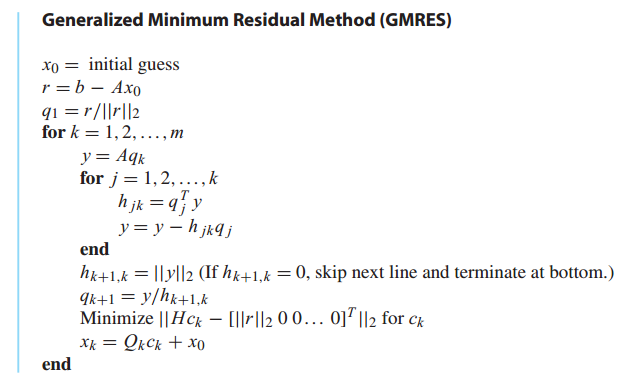
\includegraphics[width=0.7\linewidth]{gmres}
	\caption{Algorithme GMRES}
	\label{fig:gmres}
\end{figure}
\subsubsection{Résultat de l'algorithmes}

Après implémentation de l'algorithme sur python, nous obtenons des résultats assez satisfaisant. Nous avons voulu tester la robustesse de l'algorithme que nous avons implémenté. Pour cela nous avons généré plusieurs systèmes à résoudre. Afin de compliquer la tâche de l'algorithme, nous générons des problèmes, dont la taille de la matrice dépasse les 1000 lignes, sans aucun conditionnement. Pour ce faire nous générons aléatoirement les matrices en prenant des nombres entre 100 et 1000. Ensuite nous calculons l'erreur sur ce résultat par : 
\begin{equation}
\epsilon = |Ax^* - b| \text{ $x^*$ étant la solution donnée par l'algorithme }
\end{equation} 
Voici le graphique que nous obtenons : 
\begin{figure}[H]
	\centering
	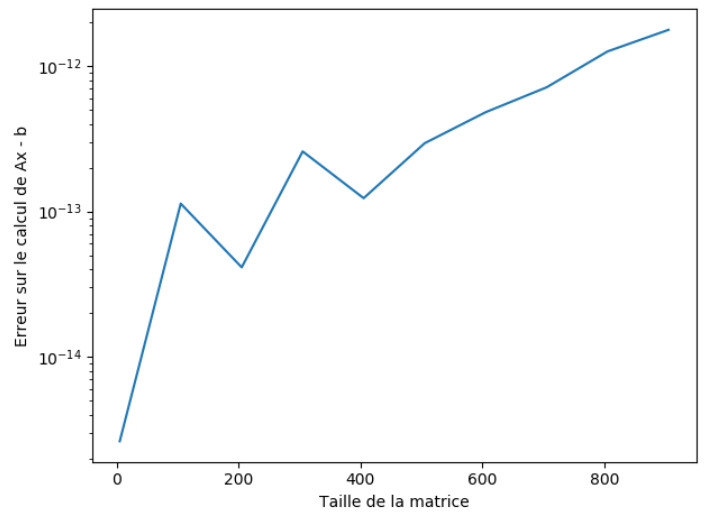
\includegraphics[width=0.7\linewidth]{err}
	\caption{Erreur sur la résolution des systèmes avec l'algorithme GMRES}
	\label{fig:err}
\end{figure}

Nous pouvons conclure de celui-ci que l'algorithme est robuste. En effet, l'erreur dans le calcul fait ci-dessus est négligeable quelque soit la taille de la matrice.